\section{Theorie}
\label{sec:Theorie}

\subsection{Fehlerrechnung}

Für die Fehlerfortpflanzung bei Gleichungen mit $N$ fehlerbehafteten Größen
wird jeweils die Formel zur Gaußschen Fehlerfortpflanzung

\begin{equation}
  \sigma = \sqrt{\sum_{i=1}^{N}\biggl(\frac{\partial f(x_i)}{\partial x_i}
  \sigma_i\biggr)^2}
\end{equation}
mit der jeweiligen Funktion $f(x_i)$, den Messgrößen $x_i$ und den
zugehörigen Fehlern $\sigma_i$ verwendet.
Zur Berechnung des arithmetischen Mittels von $N$ Messwerten wird jeweils die
Formel

\begin{equation}
  \bar{x} = \frac{1}{N}\sum_{i=1}^{N}x_i
\end{equation}
mit den Messwerten $x_i$ benutzt.
die Standardabweichung des Mittelwerts wird jeweils mit der Gleichung

\begin{equation}
  \bar{\sigma} = \sqrt{\frac{1}{N-1}\sum_{i=1}^{N}(x_i - \bar{x})^2}
\end{equation}
mit den $N$ Messwerten $x_i$ berechnet.

\subsection{Einleitung und Zielsetzung}

Das menschliche Gehör ist in der Lage, Frequenzen von ca. $\SI{16}{\hertz}$ bis
ca. $\SI{20}{\kilo\hertz}$ wahrzunehmen. Frequenzen unter dieser Hörschwelle
werden Infraschall genannt und solche, die über der Hörschwelle und unter
$\SI{1}{\giga\hertz}$ sind, werden Ultraschall genannt.
Frequenzen über $\SI{1}{\giga\hertz}$ werden als Hyperschall bezeichnet.
In diesem Versuch sollen mit Hilfe von Ultraschallwellen
Strömungsgeschwindigkeiten in einem Schlauch untersucht werden.

\subsection{Der Dopplereffekt}

Der sogenannte Dopplereffekt tritt im Allgemeinen auf, wenn sich eine
Schallquelle und ein Beobachter relativ zueinander bewegen. Die
ausgesendeten Schallwellen der Frequenz $\nu_0$, werden je nach Geschwindigkeit
in die Länge gezogen oder gestaucht, sodass die vom Beobachter wahrgenommenen
Frequenzen
verschoben sind.
Mit der Formel
\begin{align}
  \nu_{\text{q},+/-} = \frac{\nu_0}{1 + v_{\text{q},+/-}}
\end{align}
berechnet sich diese verschobene Frequenz $\nu_{\text{q},+/-}$, wenn die Quelle sich entweder
mit $v_{\text{q},+}$ zum Beobachter bewegt, oder mit $-v_{\text{q},-}$ vom Beobachter entfernt.
Wenn die Quelle sich in Ruhe befindet und der Beobachter sich mit $v_{\text{b},+}$ zur Quelle
oder mit $-v_{\text{b},-}$ von der Quelle wegbewegt, wird die verschobene
Frequenz $\nu_{\text{b},+/-}$ mit
\begin{align}
  \nu_{\text{b},+/-} = \nu_0 \Bigl(1 + \frac{v_{\text{b},+/-}}{c} \Bigr)
\end{align}
berechnet.
Der Dopplereffekt kann ausgenutzt werden, um Strömungsgeschwindigkeiten, zum
Beispiel in einem Blutgefäß, zu bestimmen. Mit einem Schallsender wird
dabei, wie in Abbildung \ref{fig:ImpulsEcho} dargestellt, ein Signal an
der Strömung ausgesendet und dann nach der Reflektion wieder am Sender
empfangen. Bei diesem sogenannten Impuls-Echo-Verfahren berechnet sich
die Frequenzverschiebung mit
\begin{align}
  \increment \nu = 2 \nu_0 \frac{v}{c} \cos{\alpha}.
  \label{eqn:deltanu}
\end{align}

\begin{figure}
  \centering
  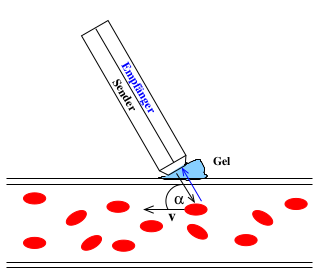
\includegraphics[height=4cm]{ImpulsEcho.png}
  \caption{Skizze zur Messung der Stömungsgeschwindigkeit mit dem
  Impuls-Echo-Verfahren. \cite{anleitung}}
  \label{fig:ImpulsEcho}
\end{figure}

\subsection{Erzeugung von Ultraschallwellen}

Ultraschallwellen können durch den sogenannten reziproken piezo-elektrischen
Effekt erzeugt werden. Dabei wird ein piezo-elektrischer Kristall durch ein
elektrisches Wechselfeld,
das in Richtung einer der polaren Achsen des Kristalls steht, angeregt und
beginnt zu schwingen und Ultraschallwellen auszusenden.
Der Kristall kann außerdem auch als Schallempfänger genutzt werden, da er auch
durch Ultraschallwellen angeregt werden kann.
